\documentclass[tikz,border=3mm]{standalone}
\usetikzlibrary{arrows.meta,calc}

\begin{document}
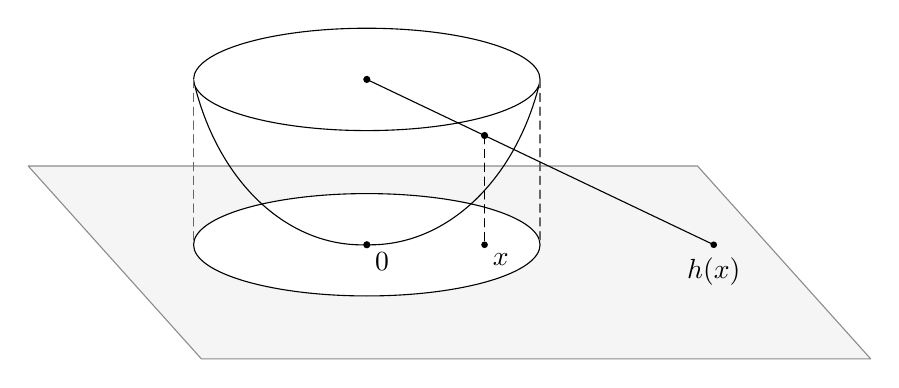
\begin{tikzpicture}[>=Stealth, line cap=round, line join=round]

% ----------------------------
% PARAMETERS
% ----------------------------
\def\a{2.2}
\def\b{0.65}
\def\H{2.1}
\def\Oy{-2.0}

\coordinate (O) at (0,\Oy);
\coordinate (Ctop) at (0,{\Oy+\H});

% ----------------------------
% BASE PLANE
% ----------------------------
% ----------------------------
% BASE PLANE (parallelogram)
% ----------------------------
\coordinate (A) at (-4.3,-1.0);
\coordinate (B) at (4.2,-1.0);
\coordinate (C) at (6.4,-3.45);
\coordinate (D) at ($(A)+(C)-(B)$); % ensures parallelogram

\path[fill=gray!8, draw=black!45]
  (A) -- (B) -- (C) -- (D) -- cycle;

% ----------------------------
% PROJECTION ELLIPSE
% ----------------------------
\fill[white] (O) ellipse [x radius=\a, y radius=\b];
\draw (O) ellipse [x radius=\a, y radius=\b];

% Center
\fill (O) circle (1.3pt);
\node[below right=-0.5pt] at (O) {$0$};

% ----------------------------
% PARABOLOID: WIRE-FRAME MERIDIANS
% z = H * r^2  with r in [0,1]
% ----------------------------

% Draw rim
\draw (Ctop) ellipse [x radius=\a, y radius=\b];
% Radial meridians (round dome instead of parabola)
\foreach \ang in {-173,-5} {
  \draw
    plot[domain=0:0.999,samples=80]
    ({\a*\x*cos(\ang)},
     {\Oy + 1.46*\H*(1 - sqrt(1 - \x*\x*0.9)) + \b*\x*sin(\ang)});
}

% \draw[densely dashed,black!60] (P) -- (x);
% ----------------------------
% VERTICAL PROJECTIONS FROM OPPOSITE TOP POINTS
% ----------------------------
\pgfmathsetmacro{\phi}{0} % choose direction

% First point on top ellipse
\pgfmathsetmacro{\xtA}{\a*cos(\phi)}
\pgfmathsetmacro{\ytA}{\Oy+\H + \b*sin(\phi)}
\coordinate (TA) at (\xtA,\ytA);

% Opposite point (phi + 180)
\pgfmathsetmacro{\xtB}{-\xtA}
\pgfmathsetmacro{\ytB}{\Oy+\H - \b*sin(\phi)}
\coordinate (TB) at (\xtB,\ytB);

% Projections on base plane
\coordinate (TAp) at (\xtA,\Oy);
\coordinate (TBp) at (\xtB,\Oy);

% Draw vertical dashed lines
\draw[densely dashed,black!60] (TA) -- (TAp);
\draw[densely dashed,black!60] (TB) -- (TBp);

% % Optional: mark the points
% \fill (TA) circle (1.2pt);
% \fill (TB) circle (1.2pt);
% \fill (TAp) circle (1.2pt);
% \fill (TBp) circle (1.2pt);


% Top point
\fill (Ctop) circle (1.3pt);

% ----------------------------
% POINT ON PARABOLOID
% ----------------------------
\pgfmathsetmacro{\rP}{0.75}
\pgfmathsetmacro{\theta}{25}

\pgfmathsetmacro{\xP}{\a*\rP*cos(\theta)}
\pgfmathsetmacro{\yP}{\Oy + \H*\rP*\rP + \b*\rP*sin(\theta)}

\coordinate (P) at (\xP,\yP);
\fill (P) circle (1.3pt);

% ----------------------------
% PROJECTION x
% ----------------------------
\coordinate (x) at (\xP,\Oy);
\fill (x) circle (1.2pt);
\node[below right=-0.5pt] at (x) {$x$};

\draw[densely dashed] (P) -- (x);

% ----------------------------
% LINE THROUGH TOP AND P -> h(x)
% ----------------------------
\pgfmathsetmacro{\yC}{\Oy+\H}
\pgfmathsetmacro{\s}{(\Oy-\yC)/(\yP-\yC)}
\coordinate (hx) at ({\s*\xP},\Oy);

\fill (hx) circle (1.2pt);
\node[below=1pt] at (hx) {$h(x)$};

\draw (Ctop) -- (P) -- (hx);

\end{tikzpicture}
\end{document}